
\begin{frame}\frametitle{How did we do it?}
  \setbeamercovered{invisible}
  \begin{columns}
    \begin{column}{0.4\linewidth}
      \begin{block}{Tasks:}
        \begin{itemize}
          \item Implement $K_{ij}$, $G_{ij}$
          \item Convenience functions
          \item 2d integration
          \item 2d interpolation
          \item Maris-Tandy
          \item Quark $M,\, A$
        \end{itemize}
      \end{block}
    \end{column}
    \pause
    \begin{column}{0.2\linewidth}
      \centering
      $\rightarrow$
    \end{column}
    \begin{column}{0.4\linewidth}
      \begin{block}{New tasks:}
        \begin{itemize}
          \item Iteration
          \item Calculate $K'_{ij}$
          \item File output
          \item Optimize
        \end{itemize}
      \end{block}
    \end{column}
  \end{columns}
  \pause
  \begin{tikzpicture}[remember picture,overlay]
    \node[anchor=south west,inner sep=0pt,text width=10cm] at ($(current page.south west)+(5.2cm,5.99cm)$) {
      \fontsize{12}{14}\selectfont\textcolor{black}{Around two days...}
    };
  \end{tikzpicture}
  \pause
  \begin{tikzpicture}[remember picture,overlay]
    \node[anchor=south west,inner sep=0pt] at ($(current page.south west)+(8.2cm,5.55cm)$) {
      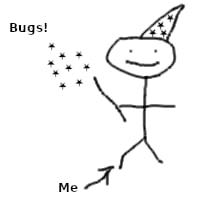
\includegraphics[width=0.17\linewidth]{Important.jpeg}
    };
  \end{tikzpicture}
  \begin{tikzpicture}[remember picture,overlay]
    \node[anchor=south west,inner sep=0pt,text width=10cm] at ($(current page.south west)+(7.2cm,1.0cm)$) {
      \fontsize{30}{35}\selectfont\textcolor{red}{\textbf{Bugs.}}
    };
  \end{tikzpicture}
\end{frame}
\endinput